\annex
\chapter{Anexo}
\renewcommand{\thesection}{\Roman{section}}
\section{Decreto 3.298  de 1999, artigo 19}
\label{decreto1}
Decreto 3.298  de 1999, artigo 19:
\begin{quotation}``Consideram-se ajudas t�cnicas, para os efeitos deste Decreto, os elementos que permitem 
compensar uma ou mais limita��es funcionais motoras, sensoriais ou mentais da pessoa 
portadora de defici�ncia, com o objetivo de permitir-lhe superar as barreiras da comunica��o e da 
mobilidade e de possibilitar sua plena inclus�o social. 
Par�grafo �nico. S�o ajudas t�cnicas: 
\renewcommand{\theenumi}{\Roman{enumi}}
\begin{enumerate}
\item pr�teses auditivas, visuais e f�sicas; 
\item �rteses que favore�am a adequa��o funcional; 
\item equipamentos e elementos necess�rios � terapia e reabilita��o da pessoa portadora de 
defici�ncia; 
\item equipamentos, maquinarias e utens�lios de trabalho especialmente desenhados ou 
adaptados para uso por pessoa portadora de defici�ncia; 
\item elementos de mobilidade, cuidado e higiene pessoal necess�rios para facilitar a 
autonomia e a seguran�a da pessoa portadora de defici�ncia; 
\item elementos especiais para facilitar a comunica��o, a informa��o e a sinaliza��o para 
pessoa portadora de defici�ncia; 
\item equipamentos e material pedag�gico especial para educa��o, capacita��o e recrea��o 
da pessoa portadora de defici�ncia; 
\item adapta��es ambientais e outras que garantam o acesso, a melhoria funcional e a 
autonomia pessoal; e 
\item bolsas coletoras para os portadores de ostomia."
\end{enumerate}
 \end{quotation}
\newpage
\section{ISO 9999:2011}
\label{iso9999}

\begin{figure}[bth!]
  \begin{center}
      \centering
      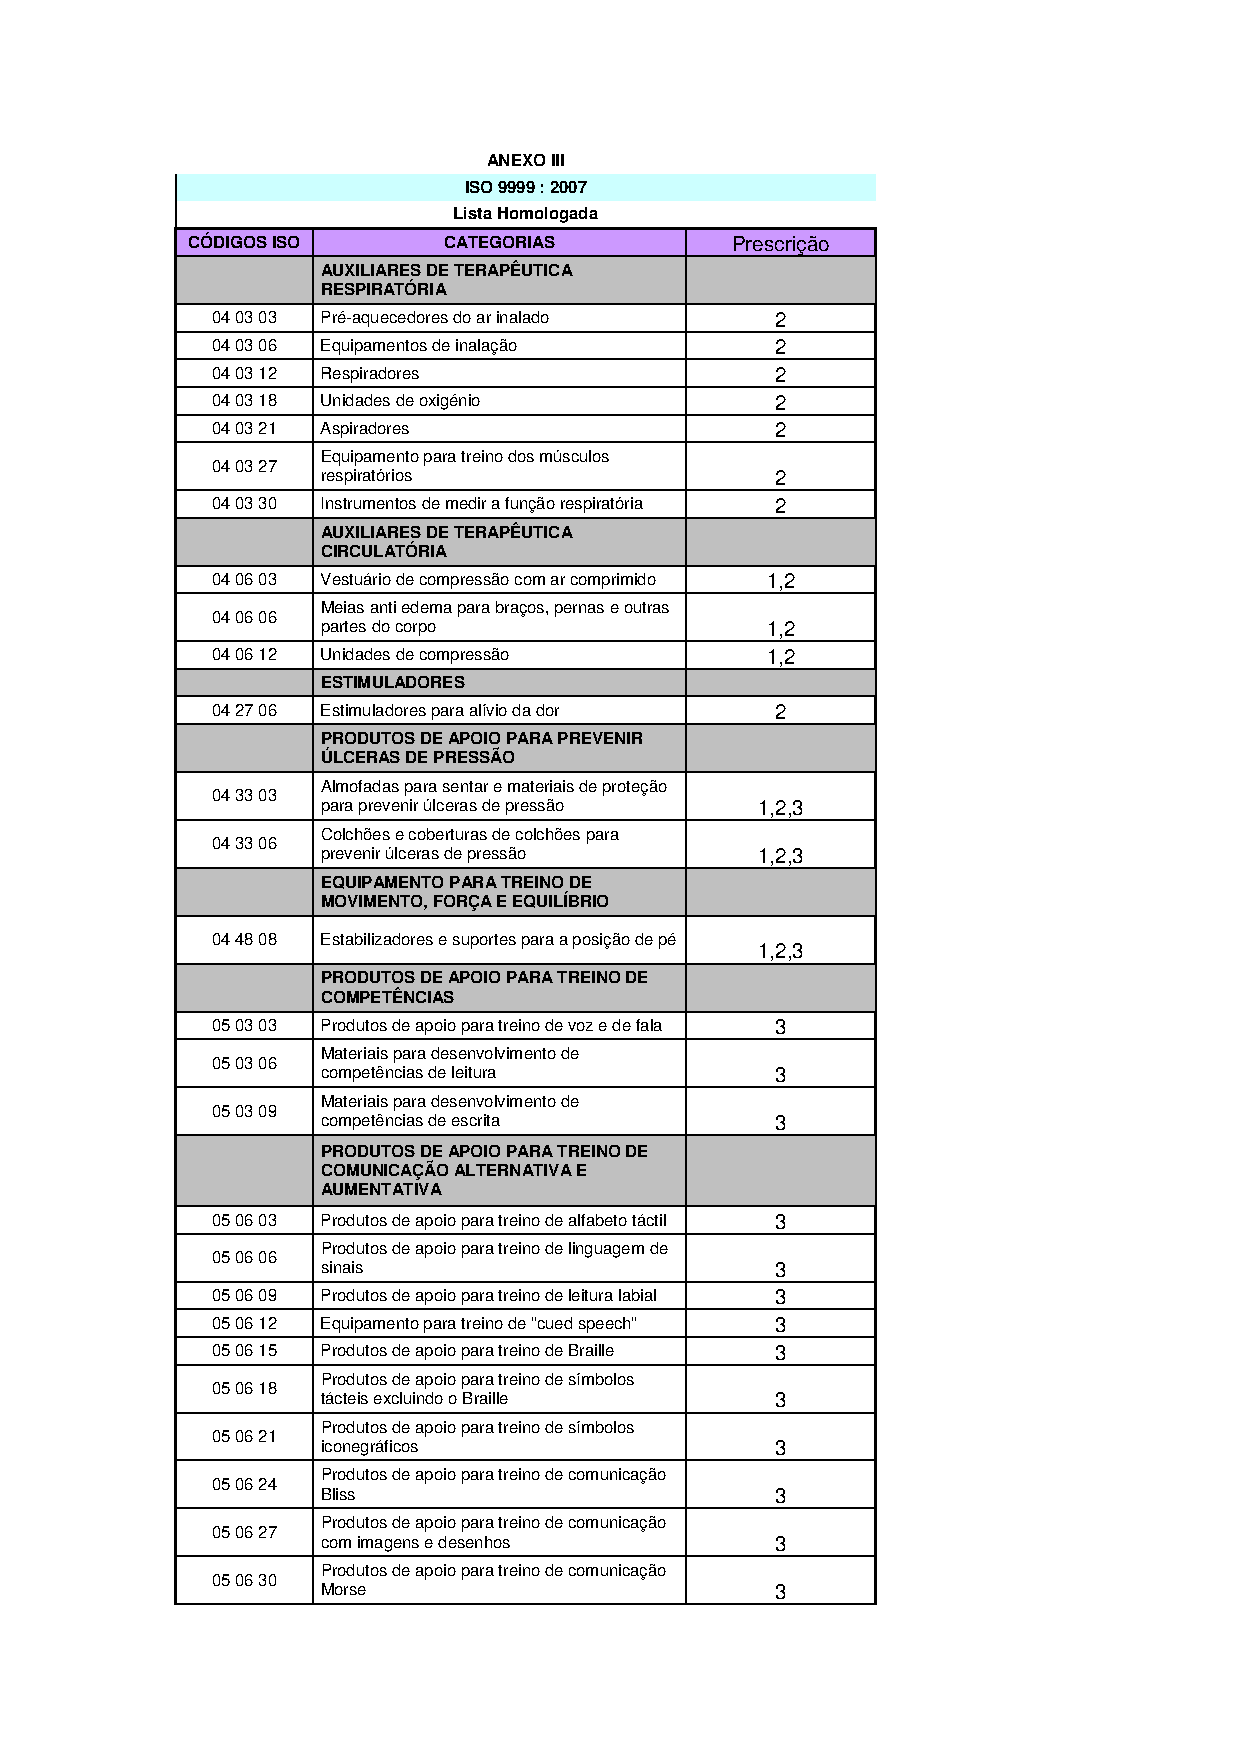
\includegraphics[page=1,scale=0.7]{../artigos/iso9999.pdf}\\
    
    \label{fig:arvore}
  \end{center}
\end{figure}
\newpage
\section{Termo de Consentimento Livre e Esclarecido}
\label{apendice2}
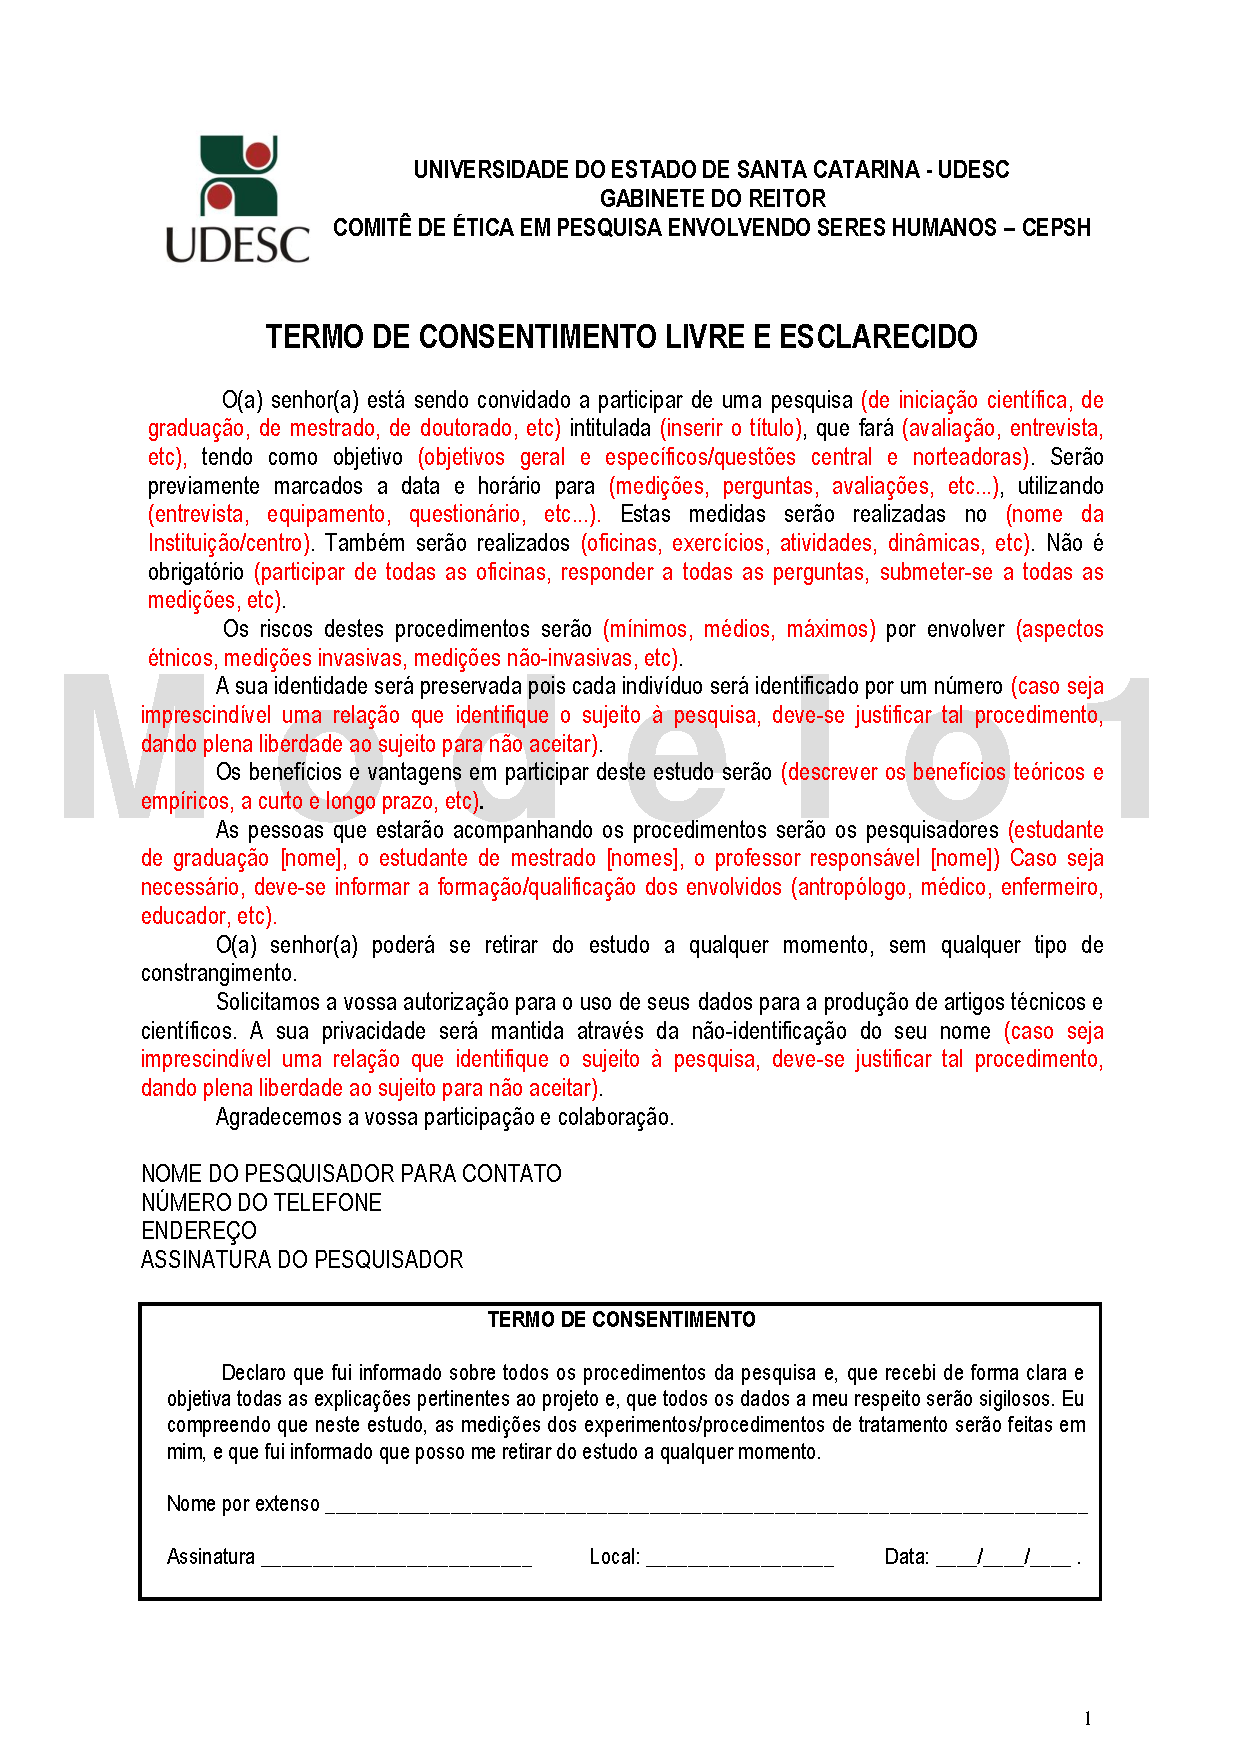
\includegraphics[scale=0.8]{../figuras/termo.pdf}
